\documentclass[
	% -- opções da classe memoir --
	article,			% indica que é um artigo acadêmico
	12pt,				% tamanho da fonte
	oneside,			% para impressão apenas no recto. Oposto a twoside
	a4paper,			% tamanho do papel. 
	% -- opções da classe abntex2 --
	%chapter=TITLE,		% títulos de capítulos convertidos em letras maiúsculas
	section=TITLE,		% títulos de seções convertidos em letras maiúsculas
	subsection=TITLE,	% títulos de subseções convertidos em letras maiúsculas
	%subsubsection=TITLE % títulos de subsubseções convertidos em letras maiúsculas
	% -- opções do pacote babel --
	english,			% idioma adicional para hifenização
	brazil,				% o último idioma é o principal do documento
	sumario=tradicional
	]{abntex2}


% ---
% PACOTES
% ---

% ---
% Pacotes fundamentais 
% ---
\usepackage{lmodern}			% Usa a fonte Latin Modern
\usepackage[T1]{fontenc}		% Selecao de codigos de fonte.
\usepackage[utf8]{inputenc}		% Codificacao do documento (conversão automática dos acentos)
\usepackage{indentfirst}		% Indenta o primeiro parágrafo de cada seção.
\usepackage{nomencl} 			% Lista de simbolos
\usepackage{color}				% Controle das cores
\usepackage{graphicx}			% Inclusão de gráficos
\usepackage{microtype} 			% para melhorias de justificação
% ---
		
% ---
% Pacotes adicionais, usados apenas no âmbito do Modelo Canônico do abnteX2
% ---
\usepackage{lipsum}				% para geração de dummy text
\usepackage{titling}
\graphicspath{{./imagens}}
\usepackage{tikz}
\usetikzlibrary{shapes.geometric, arrows}

\usepackage[scaled]{helvet}
\renewcommand*\familydefault{\sfdefault}
% ---
		
% ---
% Pacotes de citações
% ---
\usepackage[alf]{abntex2cite}	% Citações padrão ABNT
% ---


% --- Informações de dados para CAPA e FOLHA DE ROSTO ---
\titulo{Plugin de acessibilidade para sites institucionais da UFJF}
\tituloestrangeiro{Accessibility plugin for institutional websites of UFJF}

\autor{\texorpdfstring{
    João Victor Pereira dos Anjos
    \thanks{Graduando em Sistemas de Informação pela Universidade Federal de Juiz de Fora.}
    \and
    Gildo de Almeida Leonel
    }{}
}

\local{Brasil}
\data{2025}

% informações do PDF
\makeatletter
\hypersetup{
     	%pagebackref=true,
		pdftitle={\@title}, 
		pdfauthor={\@author},
    	pdfsubject={Plugin de acessibilidade para sites institucionais da UFJF},
	    pdfcreator={\LaTeX},
		pdfkeywords={Acessibilidade web}{WordPress}{WCAG}{eMAG}{Automação}{UFJF}{Inclusão digital}{Plugin},
		colorlinks=true,       		% false: boxed links; true: colored links
    	linkcolor=black,          	% color of internal links
    	citecolor=black,        		% color of links to bibliography
    	filecolor=black,      		% color of file links
		urlcolor=black,
		bookmarksdepth=4
}
\renewcommand{\author}{\raggedleft\@author}

\makeatother
% --- 

% ---
% compila o indice
% ---
\makeindex
% ---

% ---
% Altera as margens padrões
% ---
\setlrmarginsandblock{3cm}{3cm}{*}
\setulmarginsandblock{3cm}{3cm}{*}
\checkandfixthelayout
% ---

% --- 
% Espaçamentos entre linhas e parágrafos 
% --- 

% O tamanho do parágrafo é dado por:
\setlength{\parindent}{1.3cm}

% Controle do espaçamento entre um parágrafo e outro:
\setlength{\parskip}{0.2cm}  % tente também \onelineskip

% Espaçamento 1,5
\renewcommand{\baselinestretch}{1.5} % espaçamento entre linhas

\chapterstyle{article}

\usepackage{setspace}
\setlength{\parindent}{1.25cm} % Recuo de parágrafo
\setlength{\parskip}{0pt} % Remove espaçamento entre parágrafos


% ----
% Início do documento
% ----
\begin{document}

% Seleciona o idioma do documento (conforme pacotes do babel)
%\selectlanguage{english}
\selectlanguage{brazil}

% Retira espaço extra obsoleto entre as frases.
\frenchspacing

% ----------------------------------------------------------
% ELEMENTOS PRÉ-TEXTUAIS
% ----------------------------------------------------------

%---
%
% Se desejar escrever o artigo em duas colunas, descomente a linha abaixo
% e a linha com o texto ``FIM DE ARTIGO EM DUAS COLUNAS''.
% \twocolumn[    		% INICIO DE ARTIGO EM DUAS COLUNAS
%
%---

% página de titulo principal (obrigatório)
\maketitle
\thispagestyle{empty}


% titulo em outro idioma (opcional)



% resumo em português
\begin{resumoumacoluna}
    A garantia de acessibilidade digital em sites institucionais é um desafio
    crescente, especialmente em instituições públicas como a Universidade Federal
    de Juiz de Fora (UFJF). Este artigo apresenta a solução
    técnica encontrada para esse desafio, no contexto da UFJF, que é a
    implementação de um plugin WordPress para auditoria automatizada de acessibilidade,
    integrado a uma API REST externa que utiliza Puppeteer e axe-core para análise
    técnica em tempo real. O sistema permite avaliações personalizadas, focando em
    elementos editáveis por conteudistas, e gera relatórios claros com sugestões de
    correção. A metodologia abrange três etapas: análise de requisitos,
    desenvolvimento do plugin e avaliação da ferramenta. Resultados preliminares
    indicam tempos médios de resposta de 47 ms na API, relatórios traduzidos para o
    português brasileiro e adaptação às necessidades específicas da UFJF, como a
    exclusão de regras irrelevantes ao contexto dos usuários. A solução demonstra
    potencial para democratizar a fiscalização de acessibilidade, reduzindo a
    dependência de auditorias manuais e otimizando processos técnicos, ao mesmo tempo em 
    que empodera conteudistas não especialistas com dados claros e de fácil
    identificação. A proposta visa contribuir para o debate sobre automação e
    inclusão digital.

    \vspace{\onelineskip}

    \noindent
    \textbf{Palavras-chave}: Acessibilidade web. WordPress. WCAG. eMAG. Automação. UFJF. Inclusão digital. Plugin.
    \vspace{\onelineskip}
\end{resumoumacoluna}


% resumo em inglês
\renewcommand{\resumoname}{Abstract}
\begin{resumoumacoluna}
    \begin{otherlanguage*}{english}
        The guarantee of digital accessibility in institutional websites is a
        growing challenge, especially in public institutions such as the Federal
        University of Juiz de Fora (UFJF). This article presents the technical
        solution found for this challenge, in the context of UFJF, which is the
        implementation of a WordPress plugin for automated accessibility auditing,
        integrated with an external REST API that uses Puppeteer and axe-core for
        real-time technical analysis. The system allows personalized evaluations,
        focusing on elements editable by content creators, and generates clear
        reports with correction suggestions. The methodology includes three stages:
        requirements analysis, plugin development, and tool evaluation. Preliminary
        results indicate average response times of 47 ms in the API, reports
        translated into Brazilian Portuguese, and adaptation to the specific
        needs of UFJF, such as the exclusion of rules irrelevant to the context of
        users. The solution demonstrates potential to democratize accessibility
        oversight, reducing reliance on manual audits and optimizing technical
        processes, while empowering non-specialist content creators with clear and
        easily identifiable data. The proposal aims to contribute to the debate on
        automation and digital inclusion.

        \vspace{\onelineskip}

        \noindent
        \textbf{Keywords}: Web accessibility. WordPress. WCAG. eMAG. Automation. UFJF. Digital inclusion. Plugin.
    \end{otherlanguage*}
\end{resumoumacoluna}

% ----------------------------------------------------------
% ELEMENTOS TEXTUAIS
% ----------------------------------------------------------
\textual

% ----------------------------------------------------------
% Introdução
% ----------------------------------------------------------
\chapter*{Introdução}

A palavra acessibilidade é derivada do latim \textit{accessiblitas}
e significa ``condição para utilização, com segurança e autonomia,
total ou assistida, dos espaços, mobiliários e equipamentos urbanos, das
edificações, dos serviços de transporte e dos dispositivos, sistemas e meios de
comunicação e informação, por pessoa com deficiência ou mobilidade reduzida''\cite{CD}.

No Brasil, a acessibilidade é um direito garantido pela Constituição
Federal de 1988, pela Lei Brasileira de Inclusão (LBI) de 2015 \cite{LBI}
e por normas técnicas específicas, como a NBR 9050/2015 da Associação
Brasileira de Normas Técnicas~\cite{ABNT}. Essas legislações estabelecem
parâmetros para a promoção da acessibilidade em espaços públicos e privados,
visando a inclusão de pessoas com deficiência física, visual, auditiva,
intelectual e múltipla.

No âmbito digital, a acessibilidade web é um pilar fundamental para a
inclusão. O WCAG 2.1/2.2 \cite{wcag22}, sendo um conjunto de diretrizes
internacionais para a acessibilidade de conteúdo web, tem por objetivo 
tornar os sites mais acessíveis para as pessoas com deficiência visual, auditiva,
motora e cognitiva, garantindo a igualdade de acesso à informação e aos
serviços online. O eMag é um modelo nacional de acessibilidade em governo
eletrônico que estabelece diretrizes para a promoção da acessibilidade em
sites governamentais, com o objetivo de garantir a inclusão digital e o acesso
à informação para todos os cidadãos Brasileiros.

A Universidade Federal de Juiz de Fora (UFJF), como uma instituição pública,
gerencia uma grande quantidade de sites e portais, que são regularmente
atualizados por diversas pessoas, como professores, pesquisadores, bolsistas e
servidores, os quais são chamados de conteudistas. A diversidade de conteúdos e
responsáveis torna o processo de garantia de acessibilidade primordial para
atender às legislações e promover a inclusão digital.

A fim de divulgar as informações referentes aos seus setores e atividades, a
Universidade Federal de Juiz de Fora (UFJF), através do Centro de Gestão
do Conhecimento Organizacional (CGCO), é responsável por controlar a
disponibilização de sites, a padronização dos layouts e o suporte técnico. Para
a sustentação desse serviço, é utilizado o CMS WordPress~\cite{WP},
uma plataforma de gerenciamento de conteúdo que permite a criação e a 
manutenção de sites de forma simplificada e intuitiva.

Nesse cenário, há uma complexidade ao realizar auditorias manuais, que
consomem tempo e recursos, e principalmente, a falta de ferramentas
centralizadas dentro da UFJF para aplicar o Modelo de Acessibilidade em
Governo Eletrônico~\cite{emag}, conhecido como eMag, e as Diretrizes
de Acessibilidade para Conteúdo Web~\cite{wcag22}, conhecidas como
WCAG, visto que esse documentos estabelecem parâmetros técnicos para essa inclusão.

Em uma análise preliminar, avaliando a presença de elementos de acessibilidade nos
sites da UFJF, foi identificado que boa parte apresentavam falhas, como imagens sem texto
alternativo e baixo contraste de cores, limitando o acesso de usuários com deficiência
visual. Além disso, a falta de padronização e de um processo de auditoria contínuo
dificultam a identificação e a correção dessas falhas, comprometendo a qualidade e a
usabilidade dos sites.

Diante desse desafio, este artigo propõe uma solução técnica inovadora
para o contexto da UFJF, baseada em um plugin WordPress de auditoria
de acessibilidade, que integra tecnologias modernas de automação,
análise técnica e processamento de dados. O sistema opera como um serviço
independente, com suporte a regras WCAG 2.1/2.2 e eMAG, permitindo
avaliações em tempo real e personalização de regras de acessibilidade.

\chapter*{Metodologia}\label{sec:metodologia}
A metodologia proposta neste trabalho
para a implementação do sistema de auditoria de acessibilidade é dividida
em três etapas principais: análise de requisitos, onde são identificadas as
necessidades da UFJF e a realização de testes com ferramentas de acessibilidade já
existentes; desenvolvimento do plugin, onde são definidas as tecnologias a serem
utilizadas, a arquitetura do sistema, a implementação das funcionalidades e a
integração com o WordPress Multi-Sites~\cite{wp-ms}; e, por fim,
a avaliação da ferramenta,
onde são feitos testes de usabilidade, acessibilidade, desempenho e
escalabilidade do sistema.

Fragmentando a metodologia em etapas, é possível garantir um desenvolvimento
mais organizado e eficiente, com foco na qualidade e na usabilidade do sistema.
Além disso, essa divisão permite a identificação de possíveis problemas
e a realização de ajustes ao longo do processo, garantindo a entrega de um
produto final que atenda às expectativas e às necessidades da UFJF e dos
conteudistas. A seguir, será apresentada cada uma das etapas da metodologia
proposta, detalhando as atividades realizadas e os resultados obtidos.

\chapter*{Análise de Requisitos}
A primeira etapa consiste na análise dos requisitos do sistema, com base nas
necessidades da UFJF e nas diretrizes de acessibilidade. Para isso, a partir
de reuniões entre a equipe de TI e os conteudistas, chegou-se a um conjunto de
funcionalidades essenciais para o plugin, como: integração com o WordPress
Multi-Sites, avaliação em tempo real, suporte às diretrizes de acessibilidade,
relatórios claros e simples, personalização de regras a serem avaliadas e a
possibilidade de visualização de erros e sugestões de correção.

Como ja citado, ter o suporte às regras WCAG 2.1/2.2 e eMAG é fundamental para
garantir a conformidade dos sites da UFJF com as normas de acessibilidade.
Além disso, a utilização de um sistema como o CMS WordPress dentro da UFJF
é uma realidade, e portanto, a integração do plugin de acessibilidade com
essa plataforma não só é desejável, como também é essencial para garantir
que os relatórios possam ser facilmente compreendidos, visto que os
conteudistas da UFJF, responsáveis pela atualização dos sites, muitas
vezes não possuem conhecimento técnico em relação a elementos HTML,
CSS e JavaScript, o que torna relevante a disponibilização dos
relatórios de forma clara e simples, para que possam ser facilmente seguidos nas orientações sobre a
correção dos erros.

É importante ressaltar que o WordPress permite a padronização de layouts 
e que certos elementos das páginas são gerenciados pelos temas desenvolvidos pela 
equipe técnica da UFJF. Portanto, tais elementos não são passíveis de alteração
pelos conteudistas, o que torna desnecessária a avaliação de acessibilidade dessa parte. 
Sendo assim, o plugin deve permitir a
personalização tanto das regras a serem avaliadas quanto dos elementos.

Uma API REST~\cite{api}, é uma interface de programação de aplicações, que
permite a comunicação entre sistemas e é amplamente utilizada para integração
de sistemas e serviços. A utilização de uma API REST somente para a geração
dos relatórios em tempo real, sem a necessidade de armazenamento, é uma
solução mais eficiente e escalável, visto que a UFJF possui 
611 sites até abril de 2025. E armazenar os
relatórios de acessibilidade para todos esses sites em um banco de dados é tarefa que consumiria
muitos recursos e espaço em disco, tornando inviável tal abordagem.

Em fase preliminar ao desenvolvimento do projeto, realizaram-se testes com o
AccessMonitor~\cite{AM},
uma ferramenta de auditoria de acessibilidade online, que permite a avaliação de
sites em tempo real. Embora a solução ofereça uma interface intuitiva para
avaliação pontual de páginas web, identificaram-se limitações significativas para o
contexto operacional da UFJF. As principais restrições estavam na ausência de
mecanismos de personalização de regras, impedindo a adaptação a contextos
específicos, com a escalabilidade restrita e um limite operacional de páginas a
serem avaliadas por um endereço IP\@. Adicionalmente, a necessidade de inserção
manual de URLs por avaliação tornava inviável a análise de grandes portfólios de
sites\@.

Foi testada também a utilização do QualWeb~\cite{qualweb}, que é a ferramenta
de avaliação por trás do AccessMonitor. Porém, esbarrou-se em limitações técnicas,
semelhantes às encontradas no AccessMonitor, e principalmente, na falta de suporte
na tradução de relatórios para o português brasileiro, o que dificultaria a compreensão dos
conteudistas da UFJF\@.

Diante dessas limitações, optou-se por desenvolver um plugin de acessibilidade
personalizado, que atendesse às necessidades específicas da UFJF e que fosse
compatível com a infraestrutura tecnológica existente. Para auxiliar no
desenvolvimento da API REST que gerasse os relatórios de acessibilidade,
foi feita uma pesquisa por ferramentas e tecnologias que avaliassem a acessibilidade
do conteúdo DOM~\cite{DOM} de uma página web.

Foi encontrado o IBM Equal Access Toolkit~\cite{IBMa}, uma ferramenta de código
aberto desenvolvida pela IBM, que permite a avaliação de acessibilidade de páginas
web em tempo real, com suporte às diretrizes necessárias. A ferramenta oferece
o accessibility-checker~\cite{AC}, um pacote Node~\cite{Node} que permite 
testes automatizados de acessibilidade. O pacote permite também a personalização de
regras a serem avaliadas. Porém, a dificuldade de integração com a nossa API e a falta de suporte para o
português, impediu a continuidade dessa ferramenta.

Decidiu-se utilizar o axe-core~\cite{axecore}, a quarta
ferramenta de avaliação de acessibilidade que foi testada. O axe-core é uma biblioteca
de código aberto, desenvolvida pela Deque Systems, que permite a avaliação de acessibilidade
de páginas web. O ponto chave para a escolha dessa ferramenta foi a facilidade
de integração com a API REST, a possibilidade de personalização de regras a serem
avaliadas e o suporte para o português, o que facilitaria a compreensão dos conteudistas
da UFJF\@.

\chapter*{Desenvolvimento do Plugin}
A segunda etapa consiste no desenvolvimento do plugin de acessibilidade, que
integra tecnologias de automação, análise técnica e processamento de
dados. Para isso, optou-se por utilizar a linguagem de programação JavaScript, em
em conjunto com o framework Express.js~\cite{express}, um framework 
para Node.js que permite a criação de aplicações web de forma rápida
e eficiente.

Para se entender a integração com o WordPress Multi-Sites, é necessário compreender 
o conceito de Endpoints, Rotas e o que significa Multi-Sites no contexto do WordPress.
Um endpoint~\cite{endpoints} é uma URL específica que é usada para acessar
recursos em uma API, como por exemplo, uma lista de postagens ou páginas de um site. Uma
rota~\cite{routes} é um caminho específico que é usado para acessar um endpoint,
e é definido no arquivo de rotas da aplicação. O WordPress Multi-Sites é uma funcionalidade
do WordPress que permite a criação de vários sites a partir de uma única instalação,
onde cada site possui um ID único e um domínio específico, além de possuir seu próprio
conjunto de posts e páginas.

Partindo desse entendimento, o desenvolvimento do sistema foi dividido em duas partes: 
o plugin no gerenciador de conteúdo WordPress e a 
API REST hospedada em um servidor externo. O plugin é responsável por
consultar a API REST e exibir os relatórios de acessibilidade na interface do
WordPress, enquanto a API REST é responsável por receber as requisições
do plugin, avaliar a acessibilidade das páginas web e retornar os relatórios
para o plugin.

Das rotas disponíveis na API, as mais relevantes são aquelas dedicadas
à avaliação de acessibilidade: uma destinada a analisar uma página ou postagem (post)
específica e outra voltada para a verificação integral de todos os posts de um
site. Ambas compartilham um elemento central em sua estrutura: o ID do
site, que atua como parâmetro obrigatório, e a chave para identificar o contexto
da análise. Além disso, seguem um núcleo operacional comum, no qual são
acionados os processos de geração de relatórios detalhados de acessibilidade,
garantindo consistência e padronização nos resultados.

A distinção entre as duas rotas reside em um detalhe fundamental: a rota
de avaliação de um post específico possui um escopo mais restrito, focando
apenas naquele post em particular, e principalmente, é por esssa rota que
o plugin é acionado, permitindo que o conteudista realize a avaliação de
acessibilidade de um post específico e visualize o relatório na interface do
WordPress. Por outro lado, a rota de avaliação de todos os posts de um site
opera de forma mais abrangente, percorrendo todas as páginas disponíveis
e gerando relatórios. Essa diferença de escopo é essencial para atender às
demandas específicas dos conteudistas e dos desenvolvedores da UFJF.
\bigbreak

\tikzstyle{plugin} = [rectangle, rounded corners, minimum width=3cm,
minimum height=1cm,text centered, draw=black, fill=gray!30]
\tikzstyle{api} = [rectangle, rounded corners, minimum width=3cm,
minimum height=1cm,text centered, draw=black, fill=gray!30]
\tikzstyle{arrow} = [thick,->,>=stealth]
\tikzstyle{puppeteer} = [rectangle, rounded corners, minimum width=3cm,
minimum height=1cm,text centered, draw=black, fill=gray!30]
\tikzstyle{axe} = [rectangle, rounded corners, minimum width=3cm,
minimum height=1cm,text centered, draw=black, fill=gray!30]
\begin{figure}[ht]
    \centering
    \caption{Fluxo de execução da API}
    \label{fig:fluxo}
\begin{tikzpicture}[node distance=2cm]
    \node (plugin) [plugin,xshift=-2] {Plugin};
    \node (api) [api, below of=plugin] {API REST};
    \node (axe) [axe, left of=api, xshift=-3cm] {axe-core};
    \node (puppeteer) [puppeteer, below of=api] {Puppeteer};

    \draw [-latex,bend left] (plugin) edge node[anchor=west]{Url da página} (api);
    \draw [-latex,bend left] (api) edge node[anchor=east]{Relatório}(plugin);
    \draw [arrow] (api) -- node[anchor=west]{Url da página}(puppeteer);
    \draw [arrow] (puppeteer) -| node[anchor=north]{Navegador Headless}(axe);
    \draw [arrow] (axe) -- node[anchor=north]{Avaliação}(api);
\end{tikzpicture}
\end{figure}

Seguindo como base o fluxo de execução da API, apresentado na figura~\ref{fig:fluxo},
a requisição do plugin é recebida pela API REST, que se utiliza
do Puppeteer~\cite{puppeteer}, uma biblioteca Node.js que fornece uma
API de alto nível para controlar o Chrome~\cite{chrome} através do protocolo
DevTools~\cite{devtools}. O Puppeteer é utilizado para abrir uma nova aba no navegador de forma
headless~\cite{headless}, ou seja, sem interface gráfica, e carregar a URL da página
especificada na requisição. Após o carregamento da página, a API
executa a ferramenta axe-core, usando como parâmetro a página carregada
pelo Puppeteer e a personalização definida pelo CGCO, e gera uma avaliação
de acessibilidade. O resultado da avaliação é retornado para a API, que
processa o relatório, removendo informações irrelevantes e organizando os dados
para a integração com o plugin. O relatório final então é enviado de
volta para o plugin, que exibe as informações na interface do WordPress.

As principais personalizações implementadas na API serão:
\begin{itemize}
\item tradução dos relatórios para o português; 
\item regras de acessibilidade que 
não serão avaliadas por não serem passíveis de alteração pelos conteudistas;
\item diretrizes a serem avaliadas, como WCAG 2.1/2.2, ACT~\cite{ACT} e Best
Practices~\cite{BP};
\item tag HTML a ser avaliada que, para o contexto da UFJF, é o elemento que possui o conteúdo de responsabilidade do conteudista.
\end{itemize}

Entendendo o funcionamento da API e a sua importância para o
plugin, pode-se seguir para a implementação em si. O plugin WordPress
é desenvolvido em PHP~\cite{php}, uma linguagem de programação amplamente utilizada
para o desenvolvimento web, e é a linguagem utilizada pelo WordPress.

O WordPress disponibiliza a possibilidade de se adicionar elementos novos na interface
do seu gerenciador de conteúdo, através de Hooks~\cite{hooks}, que são pontos
de extensão que permitem a modificação do comportamento padrão do WordPress. Em seu
gerenciador de conteúdo, o WordPress possui uma área de administração, onde
os conteudistas podem visualizar todos os posts e as páginas do site, e editar o conteúdo
de cada um deles, representado na figura~\ref{fig:wp-admin}.
\begin{figure}[ht]
    \centering
    \caption{Área de administração do WordPress}
    \label{fig:wp-admin}
    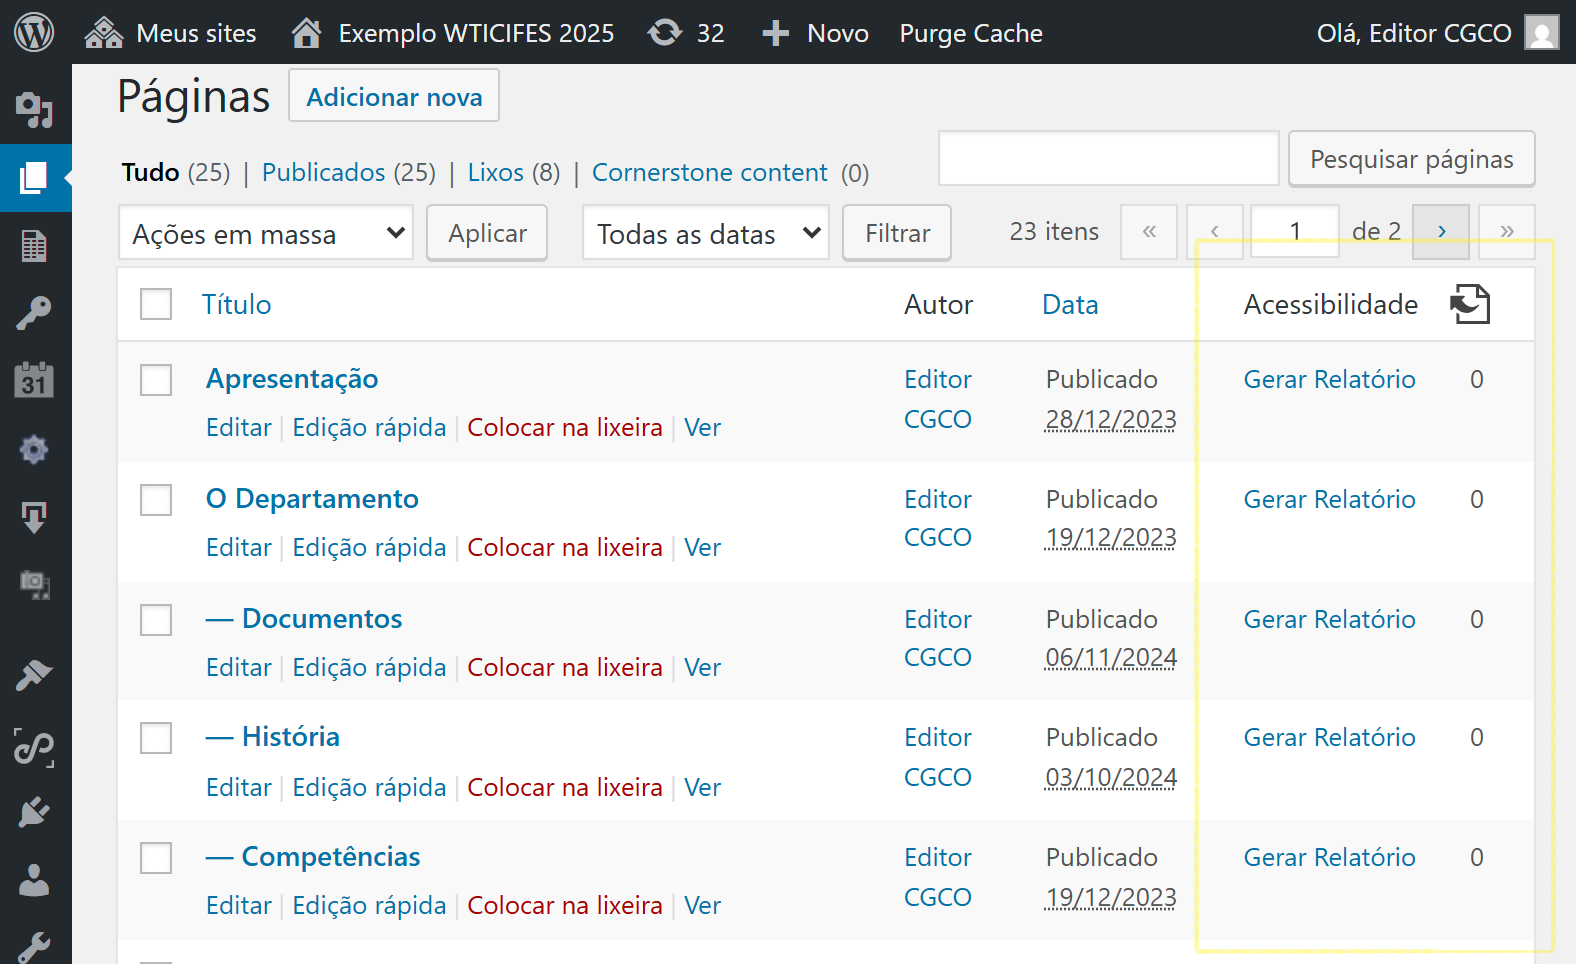
\includegraphics[width=0.7\textwidth]{imagem1.png}
\end{figure}

Tendo isso em mente, o plugin é desenvolvido para adicionar um novo botão na
interface de administração das páginas que, ao ser clicado, aciona a API REST,
passando como parâmetro a URL da página que será avaliada. O plugin aguarda a resposta da API, 
que retorna o relatório de acessibilidade. O plugin
então exibe o relatório na interface do WordPress, organizando os dados
por categoria e criticalidade, representado na figura~\ref{fig:relatorio}.

\begin{figure}[ht]
    \centering
    \caption{Relatório de acessibilidade do plugin}
    \label{fig:relatorio}
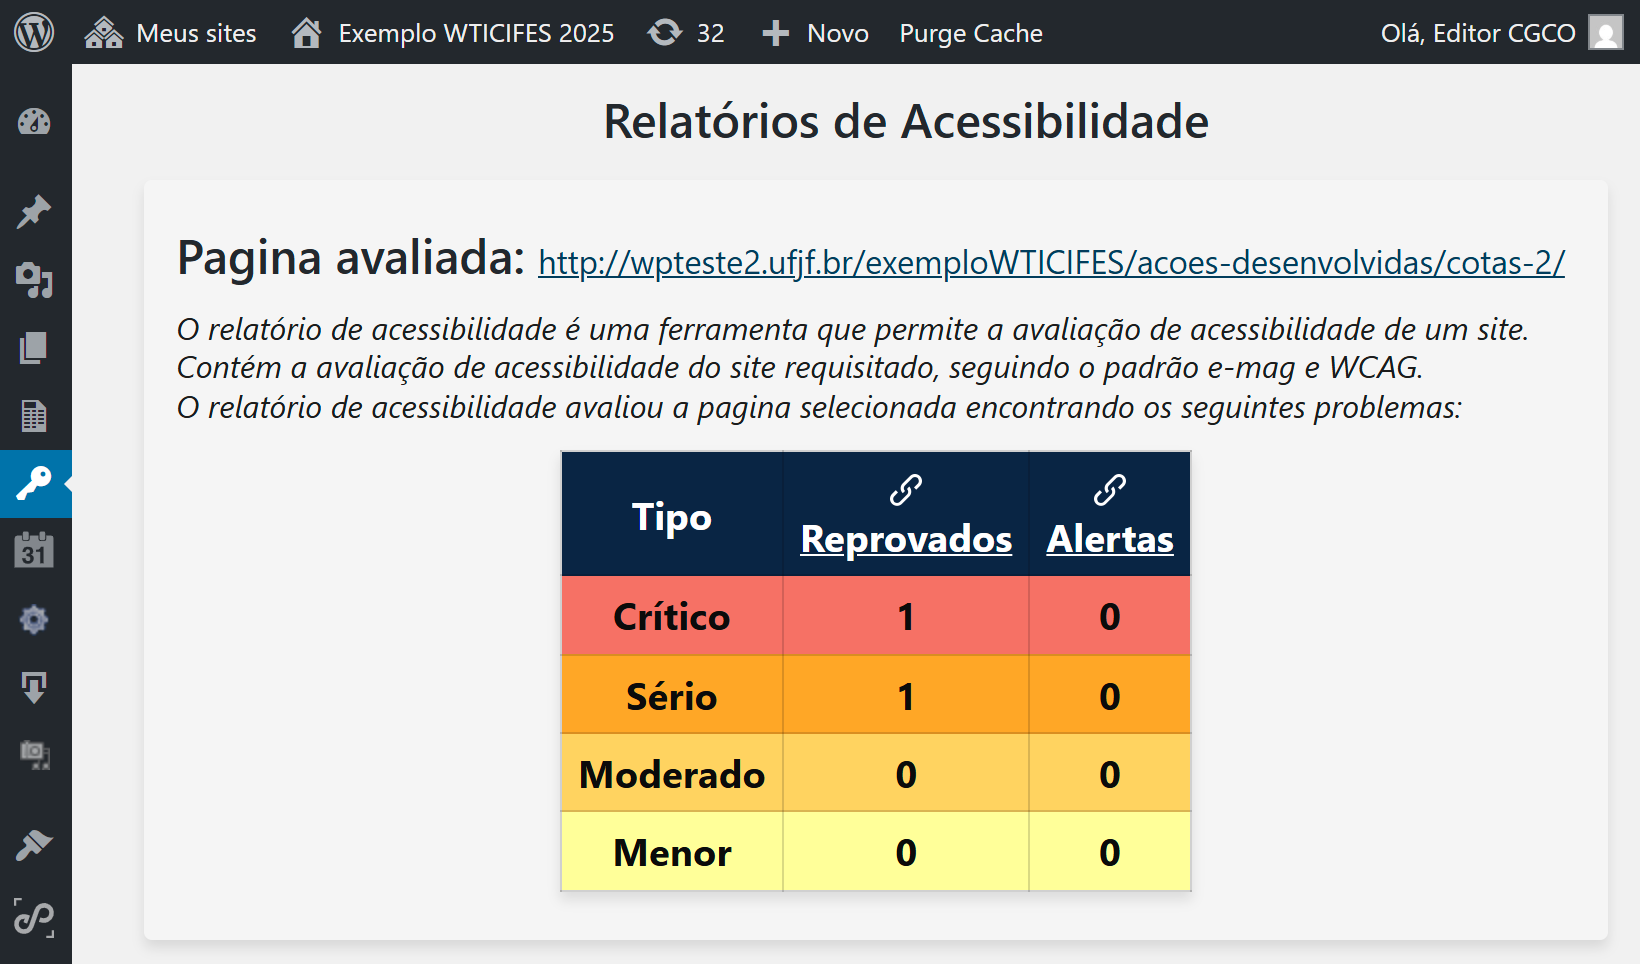
\includegraphics[width=0.7\textwidth]{imagem2.png}
\end{figure}


Em sua interface, são disponibilizadas informações
como o número de erros e os avisos encontrados,
o título da regra de acessibilidade, a descrição do erro, uma sugestão de correção 
e um link que abre a página em uma nova aba, com o elemento que apresenta o erro de
forma destacada, representado na figura~\ref{fig:relatorio2}.

\begin{figure}[h]
    \centering
    \caption{Relatório de acessibilidade do plugin}
    \label{fig:relatorio2}
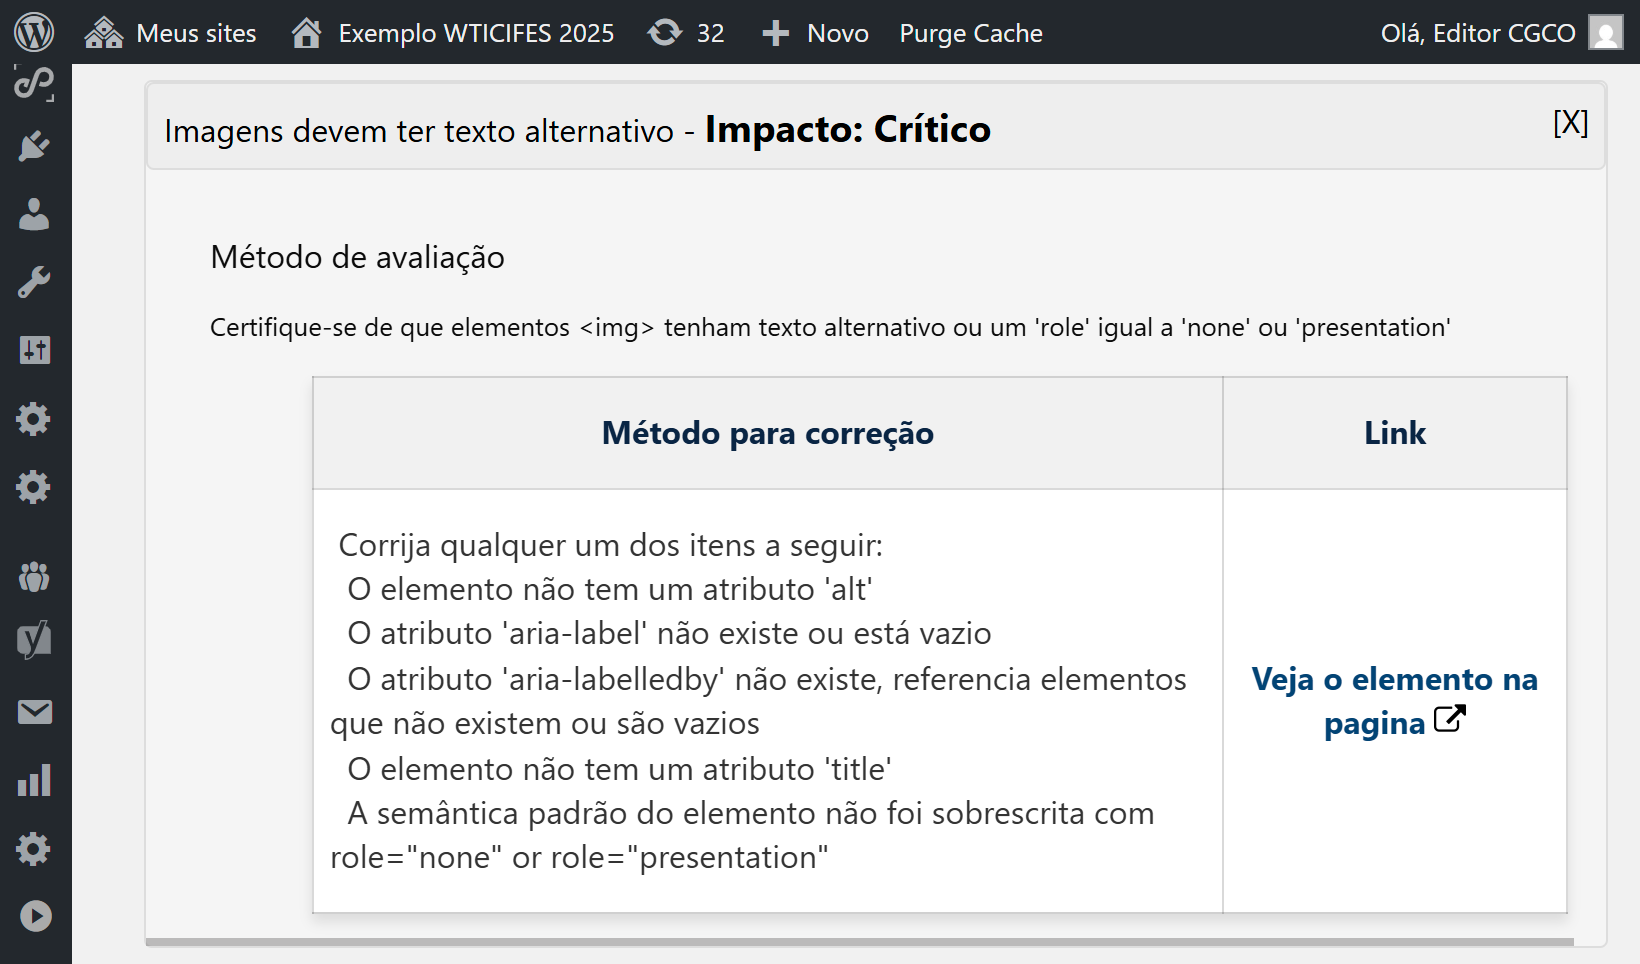
\includegraphics[width=0.7\textwidth]{imagem3.png}
\end{figure}

Dessa forma, o plugin permite que os conteudistas da UFJF possam avaliar a
acessibilidade de suas páginas de forma simples e rápida, sem a necessidade
de conhecimentos técnicos em relação a elementos HTML, CSS e JavaScript.
Além disso, o plugin permite que os conteudistas possam visualizar o que
deverá ser corrigido e como fazer isso, representado na figura~\ref{fig:relatorio3}.

\begin{figure}[h]
    \centering
    \caption{Relatório de acessibilidade do plugin}
    \label{fig:relatorio3}
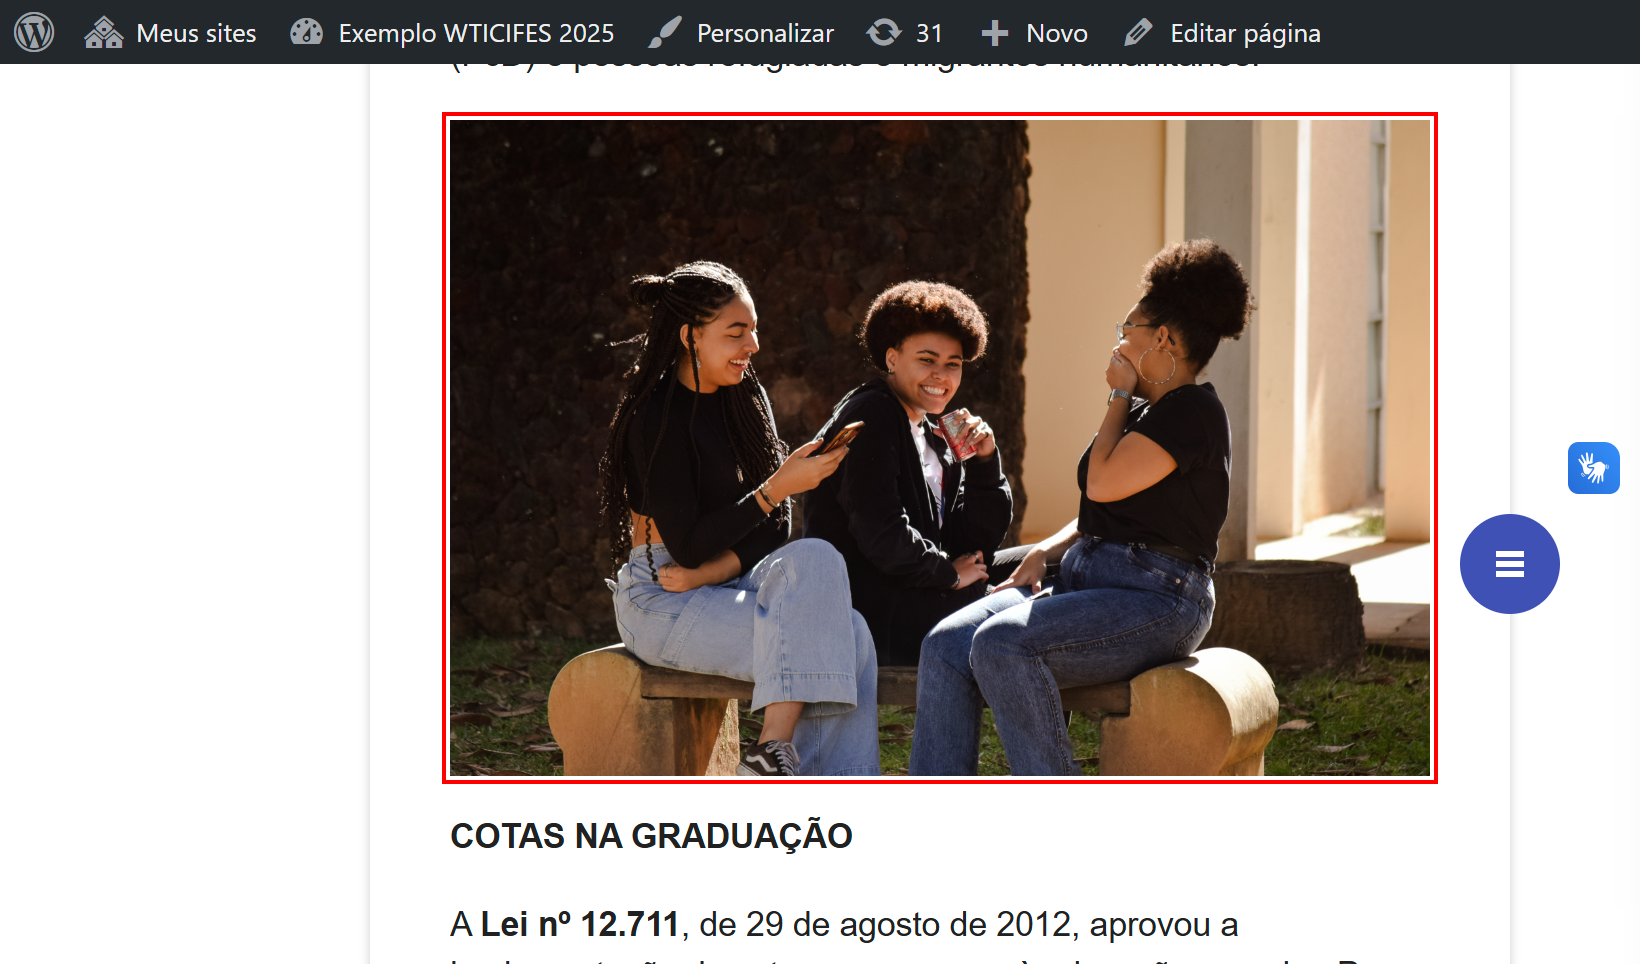
\includegraphics[width=0.7\textwidth]{imagem4.png}
\end{figure}


\chapter*{Avaliação da Ferramenta}
A terceira etapa consiste na avaliação da ferramenta, realizada 
através de testes de usabilidade, acessibilidade, desempenho e escalabilidade
do sistema. Para isso, foram realizados testes com outras ferramentas de
acessibilidade, como o AccessMonitor, para se avaliar a
confiabilidade dos relatórios gerados pelo plugin.

Durante todo o processo
de desenvolvimento, foram realizados testes de desempenho com o Insomnia~\cite{insomnia},
uma ferramenta de teste de APIs, a fim de avaliar o tempo de resposta da API. 
O tempo médio de resposta obtido foi de 47ms, o que é considerado
bom para uma API REST. Esse número foi alcançado em um ambiente
de desenvolvimento, e portanto, não reflete o tempo de resposta em um
ambiente de produção, que é variável dependendo da
carga do servidor e da quantidade de requisições simultâneas.

Além disso, serão realizados testes de usabilidade com os conteudistas da
UFJF, para se avaliar a facilidade de uso do plugin e a clareza dos relatórios
gerados. Esses testes serão cruciais para se entender quais ajustes deverão
ser feitos na interface do plugin e como melhorar a experiência do usuário.

Por fim, baseando-se em demandas internas da UFJF, foram realizados testes
de escalabilidade, para se avaliar a possibilidade de utilização da API
em outros sites da UFJF, que não são gerenciados pelo WordPress, e em outros sistemas, 
como a nova versão do SIGAx~\cite{SIGAx}, que é o sistema de Gestão Acadêmica da UFJF\@.

Com os testes de escalabilidade, foram obtidos resultados positivos, o que 
permitiu criar um novo endpoint na API para a avaliação de acessibilidade
de qualquer página web, requisitando apenas o DOM e o CSS da página, fato que foi recebido
com entusiasmo pela equipe de TI da UFJF\@. Esse novo endpoint permite que
a API possa ser utilizada em outros sistemas ainda em ambientes de desenvolvimento 
e que não estão disponíveis para o público.

\chapter*{Conclusão}
A proposta deste artigo é apresentar uma solução técnica inovadora para o
contexto da UFJF, baseada em um plugin WordPress de auditoria de acessibilidade, 
que integra tecnologias modernas de automação, análise técnica e
processamento de dados. O sistema opera como um serviço independente, com
suporte a regras WCAG 2.1/2.2 e eMAG, permitindo avaliações em tempo real
e personalização de regras de acessibilidade.

A ferramenta não apenas otimiza processos técnicos, mas democratiza
a fiscalização de acessibilidade, empoderando conteudistas não especialistas
com dados claros e de fácil identificação. Este trabalho visa, portanto, contribuir
para o debate sobre automação e inclusão digital, sugerindo um modelo que busca alinhar-se às exigências legais e éticas da
acessibilidade web, dentro do escopo do eMag, WCAG 2.1/2.2 e o contexto de cada
organização.

% \chapter*{Agradecimentos}
% Agradeço ao Centro de Gestão do Conhecimento Organizacional (CGCO) da
% Universidade Federal de Juiz de Fora (UFJF) pela oportunidade de
% desenvolver este trabalho e pela confiança depositada em mim. Agradeço
% também ao meu orientador, Gildo de Almeida Leonel, pela orientação e 
% apoio durante todo o processo de desenvolvimento do plugin de
% acessibilidade. Agradeço também a toda a equipe do CGCO, que sempre
% esteve disposta a ajudar e a contribuir com o desenvolvimento do
% plugin.

% ---

% ---
% Conclusão
% ---
% \chapter*{Considerações finais}

% \lipsum[1]

% \begin{citacao}
%     \lipsum[2]
% \end{citacao}

% \lipsum[3]

% ----------------------------------------------------------
% ELEMENTOS PÓS-TEXTUAIS
% ----------------------------------------------------------
% \postextual

% ----------------------------------------------------------
% Referências bibliográficas
% ----------------------------------------------------------
\bibliography{references}

% % ----------------------------------------------------------
% % Glossário
% % ----------------------------------------------------------
% %
% % Há diversas soluções prontas para glossário em LaTeX. 
% % Consulte o manual do abnTeX2 para obter sugestões.
% %
% %\glossary

% % ----------------------------------------------------------
% % Apêndices
% % ----------------------------------------------------------

% % ---
% % Inicia os apêndices
% % ---
% \begin{apendicesenv}

%     % ----------------------------------------------------------
%     \chapter*{Nullam elementum urna vel imperdiet sodales elit ipsum pharetra ligula
%       ac pretium ante justo a nulla curabitur tristique arcu eu metus}
%     % ----------------------------------------------------------
%     \lipsum[55-56]

% \end{apendicesenv}
% % ---

% % ----------------------------------------------------------
% % Anexos
% % ----------------------------------------------------------
% \cftinserthook{toc}{AAA}
% % ---
% % Inicia os anexos
% % ---
% %\anexos
% \begin{anexosenv}

%     % ---
%     \chapter*{Cras non urna sed feugiat cum sociis natoque penatibus et magnis dis
%       parturient montes nascetur ridiculus mus}
%     % ---

%     \lipsum[31]

% \end{anexosenv}

% ----------------------------------------------------------
% Agradecimentos
% ----------------------------------------------------------

% \chapter*{Agradecimentos}
% Texto sucinto aprovado pelo periódico em que será publicado. Último
% elemento pós-textual.

\end{document}